\documentclass{beamer}
\usetheme{Copenhagen}
\usecolortheme{default}
\usepackage{adjustbox}
\usepackage{fancyvrb}
\usepackage{float}
\usepackage{algpseudocode}
\usepackage{amsmath}
\DeclareMathOperator*{\argmax}{argmax}

%Information to be included in the title page:
\title[Gemixque - sistem de recomandări de jocuri video]{Gemixque}
\subtitle{Sistem de recomandări de jocuri video}
\author[Radu Damian]{Radu Damian \and \\[9mm] Dr. Cristian Frăsinaru}

\institute{Facultatea de Informatică}
\date{2022}

\setbeamertemplate{headline}{}
\addtobeamertemplate{navigation symbols}{}{%
    \usebeamerfont{footline}%
    \usebeamercolor[fg]{footline}%
    \hspace{1em}%
    \insertframenumber/\inserttotalframenumber
}
\begin{document}

\frame{\titlepage}


\begin{frame}
  \frametitle{Cuprins}
  \tableofcontents
\end{frame}

\section{Descrierea problemei}
\frame{\tableofcontents[currentsection]}

\begin{frame}{Privirea în ansamblu a problemei}
   Trei elemente principale:
   \begin{itemize}
  \item Utilizatorul
  \item Jocul video
  \item Recenzia
  \end{itemize}
\end{frame}

\begin{frame}{Specificații}
    Fie  \(U \)  mulțimea de utilizatori și \( G \) mulțimea de  jocuri. 
     \[ \forall  u  \in  U,  \;  \exists \; G_u \subseteq  G  \] 
     
     \[ \forall g \in G_u, \; s(u, g) = r_{ug}\]
     
     \[ 1 \leq r_{ug} \leq 10\]
     
    
    
\end{frame}

\begin{frame}{Obiectiv}
\begin{itemize}
  \item Fie \( u \in U \), \(g \notin G_u \) 
  \item \( \hat{s}(u, g) = ?\)
  \end{itemize}
\end{frame}

\section{Neo4j}
\frame{\tableofcontents[currentsection]}
\begin{frame}{Introducere în Neo4j}
    \begin{itemize}
        \item Bază de date NoSQL de tip graf
        \item Datele sunt reținute prin intermediul nodurilor și muchiilor
        \item Utilizează limbajul de interogare Cypher
    \end{itemize}
\end{frame}

\begin{frame}{Caracteristici}
    Un nod are următoarele trăsături:
    
    \begin{itemize}
        \item Reprezintă obiecte/entități
        \item Poate fi etichetat
        \item Poate avea proprietăți
    \end{itemize}
    
    
\end{frame}

\begin{frame}{Caracteristici}
    O muchie(relație) este caracterizată de:
    
    \begin{itemize}
        \item Tipul acesteia
        \item Direcția
        \item Poate avea proprietăți
    \end{itemize}
\end{frame}

\begin{frame}[fragile]{Exemplu}
    \begin{figure}[H]
        \centering
        \begin{adjustbox}{max size={\textwidth}{\textheight}}
        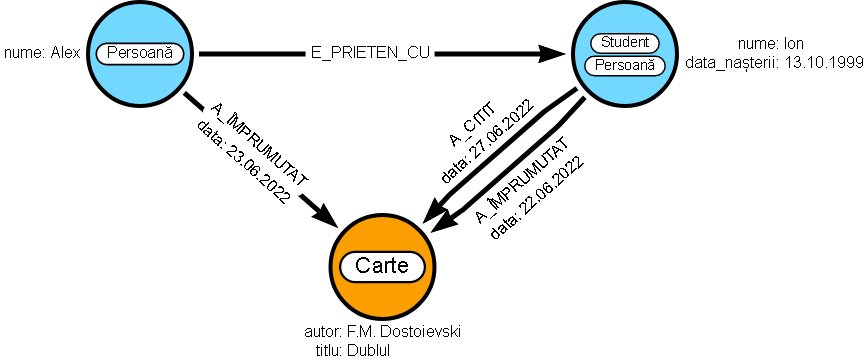
\includegraphics[scale = 0.4]{exemplu_1}
        \end{adjustbox}
    \end{figure}
\end{frame}

\begin{frame}{Limbajul de interogare Cypher}
    \begin{itemize}
        \item inspirat din SQL
        \item prezintă un mod intuitiv de reprezenta noduri și relații prin intermediul unei sintaxe tip ASCII-art
    \end{itemize}
\end{frame}

\begin{frame}{Cypher vs. SQL}
    Studiu de caz:
    \begin{itemize}
        \item modelarea situației din cadrul unei facultăți(studenți, cursuri, profesori)
        \item exemplu interogare în SQL
        \item exemplu interogare în Cypher
        \item conceptul de \emph{pattern-matching}
    \end{itemize}
\end{frame}


\begin{frame}[fragile]{Cypher vs. SQL}
    \centering
    \begin{BVerbatim}
        SELECT p.nume, p.prenume FROM NOTE n 
        JOIN CURSURI c ON n.id_curs = c.id
        JOIN DIDACTIC d ON d.id_curs = c.id
        JOIN PROFESORI p ON p.id = d.id_profesor
        WHERE VALOARE = 10 AND ID_STUDENT = 36;
    \end{BVerbatim}
\end{frame}

\begin{frame}[fragile]{Cypher vs. SQL}
    \begin{figure}[H]
        \centering
        \begin{adjustbox}{max size={\textwidth}{\textheight}}
        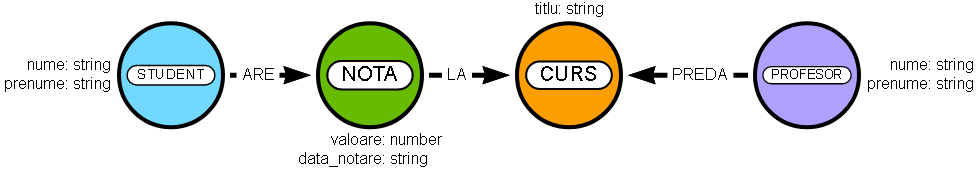
\includegraphics[scale = 0.4]{exemplu_2}
        \end{adjustbox}
    \end{figure}
\end{frame}

\begin{frame}[fragile]{Cypher vs. SQL}
    \centering
    \begin{figure}[H]
\centering
\begin{BVerbatim}
MATCH (s:STUDENT)-[:ARE]->(n:NOTA {valoare: 10}),
(n)-[:LA]->(:CURS)<-[:PREDA]-(p:PROFESOR)
WHERE id(s) = 0
RETURN p.nume, p.prenume
\end{BVerbatim}
\end{figure}
\end{frame}

\begin{frame}{Pattern-matching}
    
\begin{itemize}
    \item Conceptul de \emph{pattern-matching} este introdus prin intermediul clauzei \texttt{MATCH}
    \item În funcție de cum este definit \emph{pattern}-ul în interogare, graful va fi parcurs într-un anumit mod
\end{itemize}

\end{frame}

\begin{frame}[fragile]{Exemplu}
    \begin{figure}[H]
        \centering
        \begin{adjustbox}{max size={\textwidth}{\textheight}}
        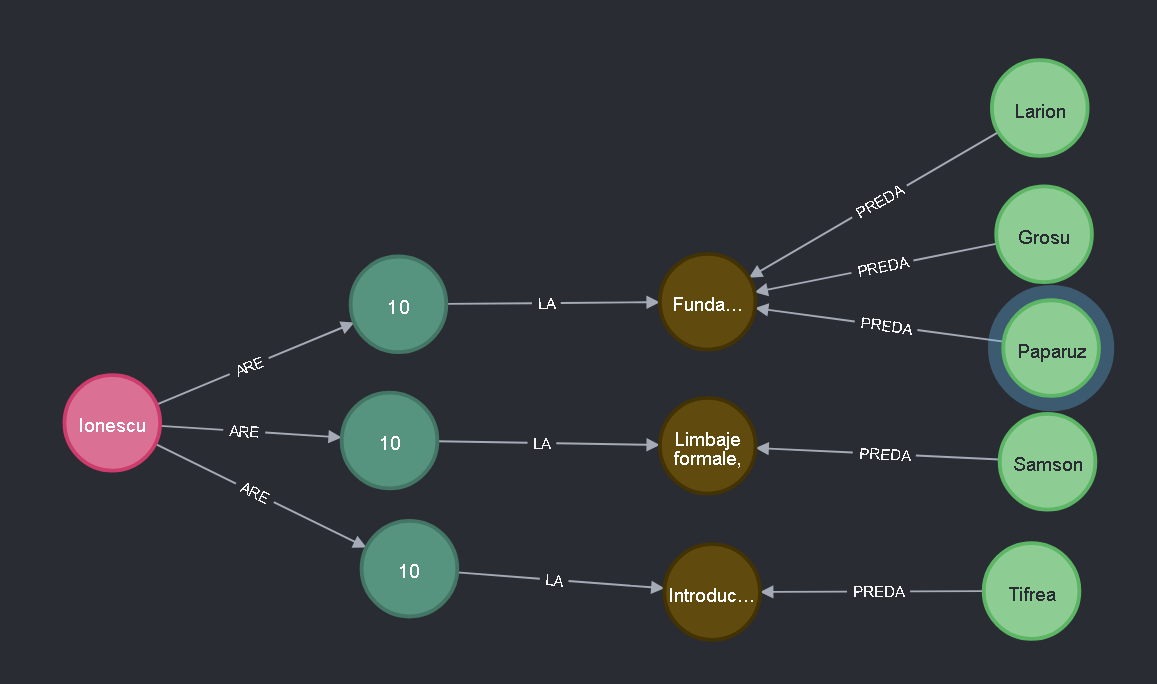
\includegraphics[scale = 0.4]{exemplu_3}
        \end{adjustbox}
    \end{figure}
\end{frame}

\begin{frame}{Schema bazei de date}
    \begin{figure}[H]
        \centering
        \begin{adjustbox}{max size={\textwidth}{\textheight}}
        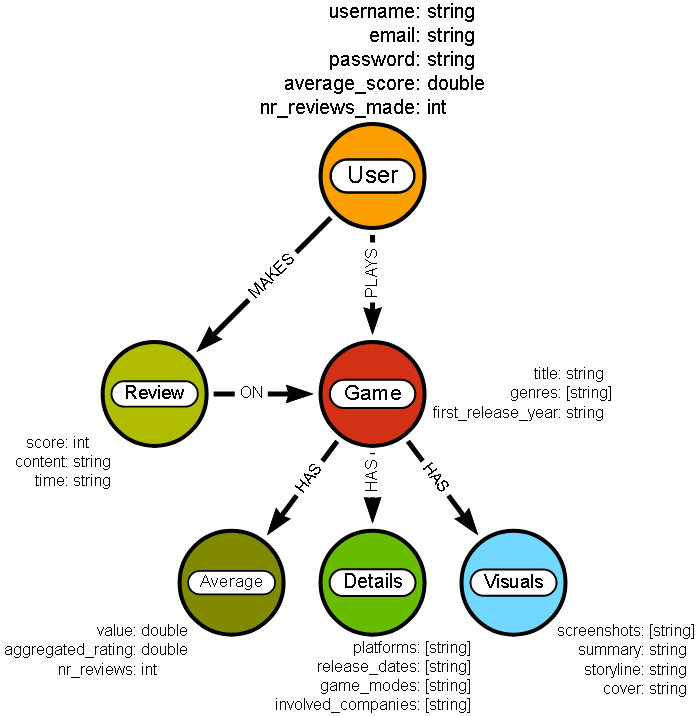
\includegraphics[scale = 0.3]{exemplu_4}
        \end{adjustbox}
    \end{figure}
\end{frame}

\section{Algoritmul de recomandare}
%Contents with current section highlighted
\frame{\tableofcontents[currentsection]}
\begin{frame}{Introducere}
 
    \begin{itemize}
        \item Ipoteză: cantitate masivă de informații
        \item Problemă: filtrarea acestor informații
        \item Solutțe: sistem de recomandare ce oferă conținut personalizat utilizatorilor
    \end{itemize}
\end{frame}

\begin{frame}{Sistem de recomandări bazat pe filtrare colaborativă}
    \begin{itemize}
        \item resurse ce nu pot fi descrise prin metadate cu ușurință
        \item matrice de scoruri utilizator-resursă
        \item calcularea unei predicții pentru elementele lipsă din matrice
    \end{itemize}
\end{frame}

\begin{frame}{Exemplu}
\begin{center}
\begin{adjustbox}{max size={\textwidth}{\textheight}}
\begin{tabular}{||c c c c c c||} 
 \hline
 & DOOM Eternal & Battlefield & Call of Duty & The Witcher 3: Wild Hunt & Dark Souls III \\ [0.5ex] 
 \hline\hline
 Ion & 9 & 8 & 10 & 3 & 6 \\ 
 \hline
 Gigel & 8 & 9 & ? & 4 & 5  \\
 \hline
 Alex & 5 & 7 & 4 & 10 & 9 \\
 \hline
\end{tabular}
\end{adjustbox}
\end{center}
    
\end{frame}

\begin{frame}{Formule}
    \[ s(u, g) = \dfrac{ \sum\limits_{u' \epsilon \Omega_{g} } w_{uu'} \cdot r_{u'g} }{\sum\limits_{u' \epsilon \Omega_{g}} w_{uu'}}  \]
    
    \( \Omega_{g}\) - mulțimea utilizatorilor care au atribuit un scor jocului \( g \)
    
    \( r_{ug} \) - nota oferită de utilizatorul \( u \) jocului g
    
    \( w_{uu'}\) - gradul desimilaritate între doi utilizatori
\end{frame}

\begin{frame}{Formule}
    \[ dev(u,g) = r_{ug} - \overline{r_{u}} \]
    
    \[ \hat{dev(u,g)} = \frac{1}{|\Omega_{g}|} \cdot \sum\limits_{u' \epsilon \Omega_{g} } dev(u', g) \] 
    
    \( \overline{r_{u}}\) - media scorurilor utilizatorului \( u \)
    
\end{frame}

\begin{frame}{Formule}
    \[ \hat{w\_dev(u,g)} = \dfrac{ \sum\limits_{u' \epsilon \Omega_{g} } w_{uu'} \cdot dev(u', g) }{\sum\limits_{u' \epsilon \Omega_{g}} |w_{uu'}|} \]
    
    \[  \hat{s}(u,g) = \overline{r_u} + \hat{w\_dev(u,g)} \;\;\; (1)  \]
\end{frame}

\begin{frame}{Coeficientul lui Pearson}
\[ w_{uu'} = \dfrac{ \sum\limits_{g \epsilon \Psi_{uu'} } dev(u, g) \cdot dev(u', g) }{
\sqrt{\sum\limits_{g \epsilon \Psi_{uu'} } dev(u, g)^2} \cdot \sqrt{\sum\limits_{g \epsilon \Psi_{uu'} } dev(u', g)^2} }\]

\( \Psi_{uu'}\) - mulțimea jocurilor în comun recenzate de utilizatorii \( u \) și \( u' \)
\( \Psi_{u}\) - mulțimea jocurilor recenzate de utilizatorul \( u \)

\( \Psi_{uu'} = \Psi_{u} \cap \Psi_{u'} \) 

    
\end{frame}

\begin{frame}[fragile]{Algoritm - pseudocod}
    \( u \in U, k \in \mathbb{N} \)
    
    getRecommendations(\(u, k \))
    \begin{algorithmic}
\State $S \gets \varnothing $

\State \textit{ submulțime de k utilizatori similari cu u ordonați descrescător după pondere:}
\State \( |U|^k \) = \( \{ X  \; | \; X \subseteq U \land |X| = k \land \argmax_{X} \sum_{x \in X} w_{ux}  \} \)

\For{\( u' \in |U|^k\)}
    \State \textit{jocuri recenzate de u' care nu sunt în comun cu jocurile recenzate de u:}
    \State \( G' = \Psi_{u'} \setminus \Psi_{uu'}  \)
    \For{\( g' \in G'\)}
        \State \( S = S \cup \{ g' \}\)
        \State actualizare scor \( g' \) utilizând formula \( (1) \)

    \EndFor

\EndFor

\end{algorithmic}
\end{frame}

\section{Concluzii}
\frame{\tableofcontents[currentsection]}
\begin{frame}{Concluzii}
	\begin{itemize}
	    \item cu ajutorul Neo4j se pot rezolva probleme în care relațiile dintre entități au o importanță semnificativă
	    \item algoritmul de recomandare prezentat reprezintă un punct de pornire în dezvoltarea în amănunt a unui sistem de recomandare
	\end{itemize}
\end{frame}

\end{document}